\documentclass[a4paper,11pt,titlepage]{scrbook}

\usepackage{graphicx}
\usepackage{fancyhdr}         % Define simple headings
\usepackage{vmargin}          % Adjust margins in a simple way
\usepackage{textpos}
\usepackage{tikz}
\usepackage{polyglossia}
\usepackage{amssymb}
\usepackage{mathtools}
\setdefaultlanguage{english}
\usepackage{unicode-math}
\usepackage{booktabs,makecell}
\usepackage[binary-units=true]{siunitx}
\usepackage[autopunct=true]{csquotes}
\renewcommand{\mktextquote}[6]{#1#2#4#3#6#5}
\usepackage[labelfont=bf,format=plain]{caption}
\usepackage{enumitem}
\setlist{itemsep=0.3ex}
\setlist[enumerate]{label = (\alph*)}
\usepackage[unicode,psdextra,bookmarksopen]{hyperref}
\hypersetup{pdfencoding=auto}
\usepackage[backend=biber,style=ieee,urldate=comp]{biblatex}
\DefineBibliographyStrings{english}{
    urlseen={accessed},
}

\DeclareFieldFormat[online]{url}{\url{#1}}
\DeclareBibliographyDriver{online}{%
  \usebibmacro{bibindex}%
  \usebibmacro{begentry}%
  \usebibmacro{author/editor+others/translator+others}%
  \newunit%
  \usebibmacro{title}%
  \newunit%
  \printlist{language}%
  \newunit%
  \usebibmacro{byauthor}%
  \newunit%
  \usebibmacro{byeditor+others}%
  \newunit%
  \printfield{version}%
  \newunit%
  \printfield{note}%
  \newunit
  \printlist{organization}%
  \newunit%
  \iftoggle{bbx:eprint}
    {\usebibmacro{eprint}}
    {}%
    %\setunit{\adddot\addspace}\newblock
  \printtext{\usebibmacro{date}}%
  \setunit{\adddot\addspace}%
  \usebibmacro{url+urldate}%
  \setunit{\adddot\addspace}%
  \usebibmacro{addendum+pubstate}%
  \setunit{\bibpagerefpunct}\newblock
  \usebibmacro{pageref}%
  \newunit\newblock
  \iftoggle{bbx:related}
    {\usebibmacro{related:init}%
     \usebibmacro{related}}
    {}%
  \usebibmacro{finentry}}

\usepackage{url}
\setcounter{biburllcpenalty}{7000}
\setcounter{biburlucpenalty}{8000}
\addbibresource{bibliography.bib}
%\usepackage{amssymb}
%\usepackage{mathtools}
\usepackage{pgfplots}
\pgfplotscreateplotcyclelist{mylist}{%
    draw={rgb,1:red,0.368417;green,0.506779;blue,0.709798},thick\\%
    draw={rgb,1:red,0.880722;green,0.611041;blue,0.142051},thick\\%
    draw={rgb,1:red,0.560181;green,0.691569;blue,0.194885},thick\\%
    draw={rgb,1:red,0.922526;green,0.385626;blue,0.209179},thick\\%
    draw={rgb,1:red,0.528488;green,0.470624;blue,0.701351},thick\\%
}

\newcommand{\docType}{Master Practicum Report} % select your thesis type
\newcommand{\mainTitle}{Evaluating the effect on countermeasures preventing the inclusion of off-topic data into Bitcoin's\\ blockchain}
\newcommand{\authorName}{Anton Ehrmanntraut}
\newcommand{\reviewerOneName}{Prof. Dr. Alexandra Dmitrienko}
\newcommand{\reviewerOneTask}{First Reviewer}
\newcommand{\advisorOneName}{}
\newcommand{\advisorOneTask}{}
\newcommand{\submissionTime}{\today}
\newcommand{\place}{Würzburg}
\newcommand{\authorDepartment}{Department of Computer Science}
\newcommand{\authorChair}{Chair of Computer Science II (Secure Software Systems)}
\newcommand{\authorAssociation}{Universität Würzburg}
\newcommand{\webadress}{www.uni-wuerzburg.de}


\addtokomafont{disposition}{\rmfamily}
\renewcommand*{\headfont}{\slshape}
\newcommand{\blankpage}{
 \clearpage{\pagestyle{empty}\cleardoublepage}
}
\setcounter{secnumdepth}{3}
\setcounter{tocdepth}{3}
\setpapersize{A4}
\setmarginsrb{3cm}{1cm}{3cm}{1cm}{6mm}{7mm}{5mm}{15mm}


\pagestyle{fancy}
\renewcommand{\chaptermark}[1]{\markboth{\thechapter.\ #1}{}}
\fancyhf{}
\fancyhead[LE,RO]{{\headfont\thepage}}						% Left/right header for even/odd pages
\fancyhead[LO]{\headfont\nouppercase{\rightmark}}	% Header for left page (odd)
\fancyhead[RE]{\headfont\nouppercase{\leftmark}}	% Header for right page (even)
\fancyfoot[C]{\thepage}
\renewcommand{\headrulewidth}{0.5pt}
\renewcommand{\footrulewidth}{0pt}
\fancypagestyle{plain}{%
\fancyhf{}													% No Header and Footer fields
\renewcommand{\headrulewidth}{0pt}
\renewcommand{\footrulewidth}{0pt}
\fancyfoot[C]{\thepage}
}

\widowpenalty 10000
\clubpenalty 10000

\hyphenation{time-stamp-ed}
\hyphenation{Block-chain}
\hyphenation{block-chain}

\begin{document}



\frontmatter
\pagenumbering{roman}
\definecolor{background}{RGB}{31,83,148}
\definecolor{titlecolor}{RGB}{255,255,255}

\begin{titlepage}

\setmarginsrb{0mm}{0mm}{0mm}{0mm}{0mm}{0mm}{0mm}{0mm}


\parindent 0cm                     % Do not indent beginning of paragraph
\parskip1.5ex plus0.5ex minus0.5ex % Margin between paragraphs


\begin{tikzpicture}[remember picture,overlay]
    \node [inner sep=0pt] (background_img) at (15, -17) {
\includegraphics[width=38cm]{logos/Marienberg_wuerzburg_verlauf.png}};
    \node [fill=white, minimum width=133mm, minimum height=600mm] (box) at (current page.north west){};
    \node [inner sep=0pt] (uniwuelogo) at (12.98,-5) {
\includegraphics[width=\paperwidth]{logos/unilogo4c_gross.png}};
\end{tikzpicture}

\pagecolor{background}

\begin{textblock*}{170mm}(55mm,15mm)
    \noindent
    \renewcommand{\baselinestretch}{1.5}
    \huge\textsf{\textcolor{titlecolor}{\docType}}
\end{textblock*}

% Title
\begin{textblock*}{130mm}(55mm,65mm)
    \noindent
    \Huge\textsf{\textbf{\textcolor{titlecolor}{\mainTitle}}}
\end{textblock*}


% First author
\begin{textblock*}{120mm}(55mm,145mm)
    \noindent
    \Large\textsf{\textcolor{titlecolor}{
    \textbf{\authorName} \\
    \authorDepartment\\
    \authorChair
    }}
\end{textblock*}

\ifdefined\advisorTwoName
	% case 1: one reviewer and two advisor
	% First reviewer
\begin{textblock*}{120mm}(55mm,190mm)
	\noindent
	\Large\textsf{\textcolor{titlecolor}{
			\textbf{\reviewerOneName} \\
			\reviewerOneTask
	}}
\end{textblock*}


% First advisor
\begin{textblock*}{120mm}(55mm,205mm)
	\noindent
	\Large\textsf{\textcolor{titlecolor}{
			\textbf{\advisorOneName} \\
			\advisorOneTask
	}}
\end{textblock*}

% second advisor
\begin{textblock*}{120mm}(55mm,220mm)
	\noindent
	\Large\textsf{\textcolor{titlecolor}{
			\textbf{\advisorTwoName} \\
			\advisorTwoTask
	}}
\end{textblock*}

\ifdefined\advisorExtName
	% external advisor
	\begin{textblock*}{120mm}(55mm,235mm)
		\noindent
		\Large\textsf{\textcolor{titlecolor}{
			\textbf{\advisorExtName} \\
			\advisorExtTask
		}}
	\end{textblock*}
\fi	
	
\else
	% case 2: one reviewer and one advisor
		% First reviewer
	\begin{textblock*}{120mm}(55mm,190mm)
		\noindent
		\Large\textsf{\textcolor{titlecolor}{
				\textbf{\reviewerOneName} \\
				\reviewerOneTask
		}}
	\end{textblock*}
	
	% First advisor
	\begin{textblock*}{120mm}(55mm,205mm)
		\noindent
		\Large\textsf{\textcolor{titlecolor}{
				\textbf{\advisorOneName} \\
				\advisorOneTask
		}}
	\end{textblock*}
\ifdefined\advisorExtName
	% external advisor
	\begin{textblock*}{120mm}(55mm,220mm)
		\noindent
		\Large\textsf{\textcolor{titlecolor}{
			\textbf{\advisorExtName} \\
			\advisorExtTask
		}}
	\end{textblock*}
\fi
\fi
% Date
\begin{textblock*}{60mm}(55mm,275mm)
    \noindent
    \Large\textsf{\textcolor{titlecolor}{\textbf{Submission\\}\submissionTime}}
\end{textblock*}

% Webadress
\begin{textblock*}{110mm}(85mm,281mm)
    \noindent
    \hfill\Large\textsf{\textcolor{titlecolor}{\textbf{\webadress}}}
\end{textblock*}

\end{titlepage}

\nopagecolor

\setmarginsrb{3cm}{1cm}{3cm}{1cm}{6mm}{7mm}{5mm}{15mm}
\chapter*{Abstract}
Blockchain-based cryptocurrencies use the blockchain data structure as persistent, distributed, append-only, and timestamped ledger.
These properties make blockchains attractive to use as storage for data that is not related to the payment processing itself.
In the case of Bitcoin's blockchain, recent studies show that this inclusion of off-topic data has already been executed in practice.
In fact, arguably objectionable content is already stored on Bitcoin's blockchain;
this potentially illegal content has the possibility to put participants of the network at legal risk, imposing a threat to the entire network.

To overcome this risk, possible countermeasures were discussed. This paper analyzes a countermeasure by Seeg, which exploits the one-way property of the address generation.
This type of countermeasure can be identified as maximally strong with respect to principles that can be considered compatible with the philosophy of Bitcoin, motivating an evaluation of the strength of this countermeasure.
By performing a brute-force exponential-time inversion on the address generation, an implementation of a circumvention is obtained.

The economic cost for executing this brute-force circumvention can be considered as a reasonable upper bound on the effectiveness of the countermeasure.
Hence, using publicly available benchmark figures, we estimate the cost of the circumvention, to assess the effectiveness of any approach attempting to prevent off-topic inclusions while adhering to the (social) principles of Bitcoin.





\tableofcontents
\blankpage

\mainmatter
\pagenumbering{arabic}
\chapter{Introduction}

Bitcoin, the decentralized, distributed, pseudonymous P2P electronic cash system introduced in 2009, makes use of blockchains, distributed data structures, as permanent tamper-proof and append-only log of transactions, enforcing irreversibility of these transactions.
By design, the blockchain is distributed inside the P2P network to all (full) nodes of the Bitcoin, and specifically every network node maintains a local copy of the entire blockchain.
While many Bitcoin users can rely on \enquote{simplified payment verification} and/or blockchain indexing servers to avoid downloading a full copy of the blockchain, full nodes – maintaining a complete up-to-date copy of the blockchain – are required in the network to independently verify the transaction ledger \cite{nakamoto_bitcoin_2008}, cf.~\cite[Chap.~8–9]{antonopoulos_mastering_2017}.

The beneficial properties of the blockchain storage – distributed, tamper-proof, timestamped, among others – have incentivized actors to use Bitcoin's blockchain as permanent storage of data unrelated to Bitcoin's payment processing.
Antonopoulos for example observes that transactions record a digital fingerprint to establish a proof-of-existence for specific files on a specific date.

The use of Bitcoin's blockchain as storage for data unrelated to payment processing is controversial, he claims.
While some see this use as abusive and worry about bloat of blockchain and payment processing, others see such (unintended) use of Bitcoin's technology as legitimate and valuable \cite[155]{antonopoulos_mastering_2017}.
Most such inclusions of off-topic data observed in practice are negligible in size and content, but nevertheless more sophisticated methods have allowed actors to include entire files such as images, or PDF files \cite{matzutt_quantitative_2018}.

Besides the issues already mentioned by Antonopoulos, the Bitcoin community observed potential legal issues in connection with this data inclusions \cite{bitcoinwiki_weaknesses_2011}, as well as the scientific community \cite{mcreynolds_cryptographic_2015}.
Illegal content in the blockchain makes participants of the network legally liable, who need to maintain a copy of the blockchain for operation.

Hence, the insertion of objectionable content has the potential to jeopardize Bitcoin (and generalizing, all blockchain-based cryptocurrencies), rendering participation illegal in certain jurisdictions.
Seeg \cite[1--2]{seeg_hardening_2018} also observes that these deliberate inclusions have the possibility to manipulate the bitcoin price, i.e.\@ expecting falling prices caused by endangered legality, and hence give an attacker serious financial incentive for executing such an attack, inserting malicious data, and profiting off, e.g.,\@ futures contracts.

Several approaches were discussed to prevent this type of off-topic data inclusion.
%These range from monitoring incoming data \cite[Sec.~IV.B]{matzutt_thwarting_2018}, consensus-based deletions of harmful portions of the blockchain \cites{ateniese_redactable_2017}{puddu_chain:_2017}, or maintaining balances instead of transactions \cite{bruce_miniblockchain_2017}.
These range from monitoring incoming data, consensus-based deletions of harmful portions of the blockchain, or maintaining balances instead of transactions, and are outlined in next section.

\subsubsection*{Approach and Contribution}

In general, we can expect that increasingly more effective countermeasures require increasingly radical methods, which in turn, make adoption of that countermeasure increasingly controversial and unlikely.
Hence, from a theoretical perspective, when given a consensus on which methods are considered so controversial that they are rejected, we can determine a maximal effectiveness of any countermeasure that is considered acceptable in the sense of the given consensus.

Due to the multitude of different interest groups and actors that constitute Bitcoin's community, a precise consensus of the approved methods available when designing an effective countermeasure seems unlikely.
Nevertheless, we can identify a minimal set of general principles that can be considered defining for Bitcoin, that is \textcquote{bitcoinwiki_prohibited_2016}{even if all Bitcoin users decide to adopt any of these changes, the resulting cryptocurrency can no longer be considered \enquote*{Bitcoin} because it has diverged too much from the original design}.

In light of these principles, we make plausible that a proof-of-ownership countermeasure, a generalization of proposed countermeasures by Seeg \cite{seeg_hardening_2018} and Matzutt et al.~\cite{matzutt_thwarting_2018}, resp., is maximally strong.
These build upon the cryptographic security of Bitcoin's key generation scheme, and requires actors to prove that they hold the private key of their respective addresses.
A brute-force exponential-time inversion on the involved cryptographic primitives leads to a trivial circumvention of that proof-of-ownership countermeasure.
Under reasonable assumptions on the one-way property of these primitives, the computational resources necessary for that specific brute-force circumvention serve as a sensible upper bound for the strength of the countermeasure.

Having established this circumvention, we focus on the main part of the paper.
As first result, a stochastic model of expected inclusion cost, in combination with a sensible estimate of the currently available computing efficiency on the cryptographic primitives, allows us to assess the effectiveness of the proposed countermeasure, and in turn by maximality, any countermeasure adhering the aforementioned principles.
Furthermore, as secondary result, we assess the impact on variations in bitcoin price and available computing efficiency on the countermeasure's effectiveness.


\subsubsection*{Outline}

Following this introduction, first Section \ref{chap:relatedwork} summarizes work related to this report's subject.
Then, Section \ref{chap:problem} gives an overview of the transaction processing in the Bitcoin network, and then demonstrates how the inclusion of off-topic data into the blockchain is currently implemented.

Section \ref{chap:countermeasure} clarifies the above-mentioned principles, which makes it immediately clear that the countermeasure proposed by Seeg cannot be further strengthened without violating the principles.
A slight generalization of his proposed countermeasure is presented, followed by an implementation of a brute-force circumvention.

On the basis of this implementation, Section \ref{chap:evaluation} establishes a stochastic model estimating the expected cost involved in executing a circumventing and inserting arbitrary data into the blockchain.
From this, the above mentioned main results are calculated.

Finally, Section \ref{chap:conclusion} concludes with a summary of the findings, and discusses potential improvements in the countermeasure.



\chapter{Related Work}\label{chap:relatedwork}

\subsubsection*{Analysis of off-topic data}

As was already outlined in the introduction, the technical problems and legal risks involved with the possibility of storing arbitrary data were recognized early on.
Hence, research focuses on one part on an analysis of currently included off-topic data in Bitcoin's blockchain; Matzutt et al.\@ \cite{matzutt_poster:_2016} quantified the found data, and in further studies \cite{matzutt_quantitative_2018} subsequently analyzed the content qualitatively on their potential legal risk, and the potential insert techniques.

These techniques were further surveyed and compared by Sward et al.\@ \cite{sward_data_2018}.
Following these results, Bartoletti et al.\@ \cite{bartoletti_journey_2019} performed an analysis on the different protocols for including data, which type of payload they include, and which techniques the respective protocols employ.

This analysis is not limited to Bitcoin's blockchain:\@
Sato et al.\@ \cite{sato_threat_2020} have begun the systematic examination of malicious files in Ethereum's blockchain.


\subsubsection*{Research into countermeasures}

In 2013, the Bitcoin development community briefly discussed some approaches to prevent the unhindered inclusion of off-topic data \cite{maxwell_prevent_2013} using the one-way property of hash functions, yet it appears that further developments were not further pursued.
These ideas were then expanded by Seeg \cite{seeg_hardening_2018} into a full countermeasure, with a patch for the Bitcoin source code as implementation.
This countermeasure is further presented and discussed in the following sections.

Independently, Matzutt et al.\@ \cite{matzutt_thwarting_2018} discussed three approaches as countermeasure:\@ (a) heuristic content detectors filtering out problematic data, (b) increasing mandatory transaction fee penalizing large transactions, and (c) \enquote{self-verifying account identifiers}, similarly exploiting the one-way property of hash functions.

Unlike the previously cited results from Seeg and Matzutt et al., this report gives a \emph{quantitative} evaluation on the effect of these proposed countermeasures.

On the other part, much research is conducted on the topic on making the blockchain mutable, to reactively remove problematic data.
Atenise et al.\@ \cite{ateniese_redactable_2017} proposed the use of intended collisions of chameleon hashes in order to implement rewriting of the blockchain.
This was further improved onto the transaction-level by Derler et al.\@ \cite{derler_fine-grained_2019}.

Puddu et al.\@ \cite{puddu_chain:_2017} presented a different approach to rewriting the blockchain, allowing the consensus-driven maintenance of alternate versions of data records, that makes any mutation controllable and verifiably by the network.
Lee et al.\@ \cite{lee_modifiable_2019} introduced an implementation of a permissionless, but modifiable blockchain using truncated hash values.

Marsalek and Zefferer \cite{marsalek_correctable_2019} improved these developments, and applied correction chains to implement a correctable blockchain architecture, which unlike the other solutions, has the capability to reduce the blockchain's set of unspent transactions.


Others approach the problem by proactively letting the network only maintain monetary information instead of a full blockchain \cite{chepurnoy_rollerchain_2016}, \cite{bruce_miniblockchain_2017}.


\chapter{Data Inclusion in the Blockchain}\label{chap:problem}

This section describes the state-of-the-art method how the transaction structure of the Bitcoin blockchain enables the inclusion of arbitrary data in the blockchain.
For this, we first outline the transaction processing of the Bitcoin network on the basis on its scripting language. Then, describes the techniques how this structure can be exploited for data inclusion, and sensibly restrict our considerations on one specific technique type.


\section{Transaction Structure and Processing}

In the Bitcoin network, the transfer of electronic coins is realized using \emph{transactions}.
From a structural perspective, every transaction specifies a set of \emph{transaction inputs} and a set of \emph{transaction outputs}, with every input referencing a previous transaction's output.
Following these references, each transaction can be considered as a vertex of a directed acyclic graph, where  its references the directed edges. Sinks of that graph correspond to (mined) coinbase transactions.

To give this transaction authenticity, an eligible user attaches to each reference some form of digital signature.
By verifying each signature associated with the preceding transactions in the graph, one can follow and verify the chain of ownership of the coins.
Hence, strictly speaking, \textquote*{ownership of coins} in the Bitcoin network is the ability to create a transaction referencing outputs not already referenced, using ownership of private keys to generate valid signatures.
Using the blockchain as a timestamping server prevents double-spending of transaction outputs.

Bitcoin implements the authenticity system of these references using a challenge–response authentication between the referenced transaction outputs and the transaction inputs.

\begin{itemize}
    \item Every output contains a \emph{locking script}, which can be understood as the cryptographic puzzle or challenge, which was defined when the transaction was constructed.
    \item A reference to an output from an input is authentic if the corresponding \emph{unlocking script} can solve the challenge imposed by the referenced output.
\end{itemize}

Bitcoin provides several methods for implementing locking and unlocking scripts, and as example, the widespread pay-to-public-key script types are presented: In this scenario, a payee Bob expects the payer Alice to publish a valid transaction with his public key embedded in the locking script of an output $x$.
Then, to transfer these coins to Charlie, Bob constructs a transaction $t$ with an input referencing $x$, adding to the unlocking script a signature of message $t$, signed with his private key, corresponding to the public key embedded in $x$.
Then Bob can add the output with the locking script expected by Charlie, and submit the transaction; cf.\@ \cite[Chap.~6--7]{antonopoulos_mastering_2017}.


The network verifies this reference by checking the signature of the unlocking script against the public key embedded in the locking script $x$.


Bitcoin employs an \emph{Elliptic Curve Digital Signature Algorithm} (using parameters from SEC2-secpk256k1) as implementation of a public-key system.
Henceforth, we refer to $G\in \mathbb{F}_p^2$ as the base point of the elliptic curve group (over the finite field of prime order $p$). For $x\in \mathbb{N}$, let $x\cdot G$ denote the elliptic curve point multiplication by a scalar.

Table \ref{table:script-types} summarizes the five standard locking script types (i.e.\@ address types) with their corresponding unlocking script. Any other forms of locking scripts are currently rejected by network participants.
Hash function $H$ is implemented in Bitcoin as composition of first SHA256, followed by RIPEMD160.

\begin{table}
    \renewcommand{\arraystretch}{1.2}
    \centering
    \begin{tabular}{lll}
        \toprule
        \textbf{Type} & \textbf{locking script\,/\,address} & \textbf{unlocking script} \\
        \midrule
        P2PK & pubkey $x\cdot G$ & sig of tx from privkey $x$ \\
        P2PKH & hash of public key $H(x\cdot G)$ & $x\cdot G$, sig of tx from $x$ \\
        P2MS & pubkeys $x_1{\cdot} G, x_2{\cdot} G, \dots, x_n{\cdot} G$ & sigs of tx from $x_{i_1}, \dots, x_{i_m}$ \\
        P2SH & hash $H(s)$ of redeem script $s$ & $s$ plus additional data $y$ \\
        Null Data & $\leq \SI{80}{\byte}$ arbitrary data & (unspendable)\\
        \bottomrule
    \end{tabular}
    \caption[Overview of the discussed standard address types]{Overview of the discussed standard address types: P2PK (pay-to-public-key), P2PKH (pay-to-public-key-hash), P2MS (pay-to-multisig), P2SH (pay-to-script-hash), Null Data. For pay-to-multisig (P2MS), $1\leq m\leq n\leq 3$ is required to be considered standard. See following text for a definition of redeem script.}
    \label{table:script-types}
\end{table}

The P2SH (pay-to-script-hash) type requires further explanation: this address type is a generalization of the challenge–response authentication employed by the network, and allow users to create their own challenges and responses using a limited scripting language.
A locking script consists of the hash of the challenge script $s$ (called \emph{redeem script}), while the unlocking script must contain the corresponding redeem script (transferred out-of-band to the payee), and additional parameters $y$ that the author of the redeem script $s$ requires as input to $s$ to be processed, checking authenticity of the payee, i.e.\@ $s$ accepts on input $y$.




\section{Script-Based Data Inclusion}\label{sec:fakekeys}

As was introduced above, the Bitcoin network employs a blockchain as a distributed data structure to prevent double-spending of transaction outputs, i.e.\@ multiple references to the same output.
The blockchain acts as timestamping mechanism, by providing \textcquote[307]{nakamoto_bitcoin_2008}{a system for participants to agree on a single history on the order \textins{of transactions} in which they were received}, hence storing every transaction with its relevant information in that data structure on time of submission.

This data structure disallows any modification on the agreed set of transactions \emph{by design}, to maintain the chain of ownership induced by the transactions.
Hence, the locking and unlocking scripts of every transaction are stored in the blockchain, essentially indefinitely, and distributed to each participant to verify the chain of ownership.

\subsubsection*{Inclusion on Outputs\,/\,Locking Scripts}

Null Data transactions already give actors the possibility to create (unspendable) transactions that contain up to \SI{80}{\byte} of arbitrary data payload. This imposed size limit is deliberately low to limit blockchain bloat, and to make this inclusion costly and not suitable for large quantities of data; cf.\@ \cite[155--156]{antonopoulos_mastering_2017}.

Therefore, more sophisticated techniques for data inclusion build upon the fact, that the network does not, and cannot test if the variable parts of the locking scripts, e.g.\@ pubkey(s) $x\cdot G$ in P2PK (P2MS) transactions, hashes $H(x\cdot G)$, $H(s)$ in P2PKH, P2SH transactions, are in fact, generated using the usual intended way.
For example, consider payload $y$ of \SI{65}{\byte}.
The network accepts and stores a P2PK transaction with $y$ as \textquote*{fake} public key masquerading as such in its locking script, even though $y\neq x\cdot G$ for all $x$ (in fact, even if $y$ does not conform to the syntax of an EC point).
Again, this means that the coins \textquote*{sent} to the fake address $y$ cannot be spent, i.e.\@ coins \emph{burnt}, just as it is the case of Null Data transactions.
Unlike Null Data outputs, a multitude of P2PK outputs can be present in a transaction, making the technique using P2PK outputs more cost-efficient.
Refer to the paper of Sward et al.\@ \cite{sward_data_2018} for an in-depth discussion of efficiencies using these techniques.

\subsubsection*{Inclusion on Inputs\,/\,Unlocking Scripts}
While the previously presented inclusion techniques insert their payload in the locking scripts, Sward et al.~\cite{sward_data_2018} analyzed inclusion approaches using P2SH unlocking scripts.
Again considering payload $y$, they construct a specialized redeem script $s$ and unlocking script $s'$, such that $y$ is a substring in $s'$.
To now perform the inclusion into the blockchain, first one publishes a transaction containing P2SH output with $H(s)$, then another transaction referencing this output, containing $s'$ as unlocking script.
This results in two valid transactions, and even require no burnt coins.
In fact, Sward et al.\@ showed that this technique outperforms every known inclusion technique using locking scripts, given the fact that unlocking scripts have a much higher size limitation in comparison to locking scripts, which have a fixed format.

Nevertheless, we will exclude an analysis of this inclusion technique in this report.
These complex transaction types might be the easiest to ban or limit, if data inclusion using P2SH inputs were to become a problem.
Since most P2SH transaction effectively implement a multisig scheme, a consensus for imposing a fixed structure for redeem scripts might be established, especially if data inclusion using unlocking scripts causes major threats.



\chapter{Countermeasure and Circumvention}\label{chap:countermeasure}

The following section first gives a detailed definition of the proof-of-ownership countermeasure. After specifying the functionality and demonstrating its intended effect, we develop an efficient brute-force method to circumvent this countermeasure. The last part of the section gives details on how to implement such circumvention in practice.

A straightforward idea for preventing data inclusion would make the network \textquote*{forget} stored information after processing, or allow the network to remove undesirable data, or recognize bad transactions using a heuristic, before they are distributed and stored; cf. the approaches from Section~\ref{chap:relatedwork}.
However, all these preventions conflict with certain properties of the network, that are universally considered characterizing for the Bitcoin system.
Hence, the adoption of such countermeasure would transform the Bitcoin system to such an extent, that the resulting electronic cash system would in general not be considered \textquote*{Bitcoin}.

While there is no central authority stating these properties, the corresponding \emph{Bitcoin Wiki} text can serve as a representative for the consensus of the community:
\begin{quote}
    \noindent\textooquote
    All changes and upgrades to the protocol should strive to maintain and reinforce these Principles of Bitcoin

    \begin{enumerate}[label={[}\arabic*.{]}]
        \item 21 million coins.
        \item No censorship: Nobody should be able to prevent valid txs from being confirmed.
        \item Open-Source: Bitcoin source code should always be open for anyone to read, modify, copy, share.
        \item Permissionless: No arbitrary gatekeepers should ever prevent anybody from being part of the network (user, node, miner, etc).
        \item Pseudonymous: No ID should be required to own, use Bitcoin.
        \item Fungible: All coins are equal and should be equally spendable.
        \item Irreversible Transactions: Confirmed blocks should be set in stone. Blockchain History should be immutable\textcoquote{} \cite{bitcoinwiki_principles_2017}.
    \end{enumerate}
\end{quote}
The mentioned countermeasures above would contradict principles 4, 7, at least.

Hence, we continue our analysis only on countermeasures that are compatible with these properties, since all nonconforming countermeasures might face serious opposition to adoption from the community.
From these principles appear to follow, that these countermeasures must respect following propositions, when determining if a submitted transaction contains no bad data:
\begin{enumerate}
    \item Every honest user can convince the system implementing the countermeasure in question that its submitted transaction is not bad, without relying on third parties, i.e.\@ using only the private key (by principle 2, 5, 6).
    \item Further assessment needs to be made transparently, especially without an authoritative figure (by principle 4),
    \item it needs to be made \emph{before} publication of the transaction (by principle 7).
\end{enumerate}
As a consequence of (a), honest addresses are those derived from a private key, as otherwise, proof asserting honesty requires a third party.
This implies that all addresses possible to generate are clean in general.
While (b) and (c) could allow for further consensus-approved content filters deciding which addresses are clean, the decentralized nature of the Bitcoin network, together with (b) and (c), make efficient filters particularly hard to implement.

Hence, without loss of generality, we need to assume a submitted destination address as clean if the owner of that address can prove the existence of the corresponding private key, that is, ownership of the address.

Matzutt et al.\@ \cite[Sec.~III.C]{matzutt_thwarting_2018} already pointed out that, under this setup, pseudonymous identifiers (cf.\@ principle 5) always open the possibility to insert data by encoding them into these identifiers: no matter how \textquote*{existence of the private key} is implemented, users willing to insert content into the blockchain always have the possibility to generate arbitrarily many addresses until suitable ones encoding the content are found.

Following section introduces a proof-of-ownership countermeasure that appears to be the strongest one respecting these propositions, motivating the evaluation of this countermeasure and its circumvention, which directly incorporates the approach outlined by Matzutt et al.


\section{Proof-of-Ownership Countermeasure}

In his Master's thesis \emph{Hardening Bitcoin against off-topic data inclusion}, Seeg proposes a countermeasure to this problem using a proof-of-ownership mechanism, which he calls \textquote{preimage solution} \cite{seeg_hardening_2018}.
He considers an address clean (i.e.\@ without arbitrary data) if and only if the owner of that address can prove control, that is, ownership of the address.
Such proof of ownership is derived from the \textquote*{private} preimage part of the address, similar to a classic challenge–response authentication.
The wanted effect follows from the assumption that given \textquote*{public} part of a non-clean address, one cannot efficiently derive \textquote*{private} preimage required for the proof of ownership.

For P2PK address types, this translates into a proof using signatures, which certify the control of the corresponding private key.
That is, in order for Alice to send coins to Bob, he sends her out-of-band his public key $x\cdot G$, and – this is the addition of the countermeasure – a signature $\sigma$ verifying message $m=H(x\cdot G)$, generated using private key $x$.
This signature proves that Bob is in control if his private key.
Then, Alice can construct a P2PK transaction with recipient key/address $x\cdot G$, and when submitting the transaction to the network, she attaches $\sigma$ which proves that Bob indeed controls that address.
(This entails that $\sigma$ needs to be transmitted out-of-band to Alice before the transaction.)
Miners can verify $\sigma$ using the public key $x\cdot G$ embedded in the transaction, approving the output address of the transaction.

This countermeasure protects against data inclusion: if an adversary wishes to embed message $y$ as public key, he cannot efficiently derive $x$ such that $x\cdot G = y$, required in order to sign the proof $\sigma$.
Thus, given valid $\sigma$, the transaction in question can be safely included into the blockchain.

In the case of P2PKH and P2SH addresses, proofs are constructed similarly.
For P2PKH addresses $H(x\cdot G)$, signed message $m$ remains identical.
Only the public key $x\cdot G$ is additionally transferred such that $\sigma$ can be verified by the network.
For P2SH addresses $H(s)$, the redeem script $s$ serves as preimage/proof $\sigma$.
Again, this prevents data inclusion due to the one-way property of hash function $H$.

Note that in the case of P2PKH and P2SH transactions, Seeg proposes to exploit the definition of $H=\mathrm{SHA256}\circ\mathrm{RIPEMD160}$: the image $\sigma = \mathrm{SHA256}(s)$ serves as proof of ownership for $H(s)=\mathrm{RIPEMD160}(\sigma)$.
Nevertheless, without loss of generality we can abstract away from that specific implementation and focus on \enquote*{full} preimages as defined in previous paragraph, since Seeg's approach identically relies on the one-way property.

In fact, the proposed countermeasure appears to be one of the strongest compatible with the Principles of Bitcoin.
We already observed that existence of a private key needs to be taken as sufficient proof that the public address is clean, and this countermeasure appropriately takes respective signatures $\sigma$ as such proof of existence.
Addresses that withstand the proposed test hence are precisely the addresses that are derived from private keys.

Additionally, other countermeasures that respect these mentioned principles build on top of the one-way property of the same cryptographic functions in a similar matter, e.g.\@ \textquote{self-verifying account identifiers} proposed by Matzutt et al.\@ \cite[Sec.~IV.D]{matzutt_thwarting_2018}.
Therefore, this countermeasure and the respective circumvention act as representative for all one-way-based approaches.

\section{Circumvention Using Partial Preimages}\label{sec:circumvention}

In essence, the proposed countermeasure builds upon preimage resistance of the cryptographic functions translating a private key into a public address.
That is, for given address derivation function $f$, required preimage $x$ for the proof-of-ownership cannot be efficiently derived from image $f(x)$, whereas only $f(x)$ is stored in the blockchain.
Attempts to embed chosen $y$ as address into the blockchain hence become computationally hard, since finding $x$ such that $f(x)=y$ is required.
For given address type, the address derivation function $f$ is precisely the procedure translating a private key into the locking script, as outlined in Table \ref{table:script-types}.
From the implementation follows, that the countermeasures builds upon the (presumed) one-way property of hash function $H$ (in the case of P2SH, P2PKH addresses) and elliptic curve multiplication (in the case of P2PK, P2MS addresses).

No matter the chosen function $f$, the trivial approach to find a preimage to value $y=f(x)$ is via \emph{brute force}: we test pairwise different preimage candidates $x_1, x_2, \dots$ until we find $x_i$ such that $f(x_i)=y$.
The preimage $x_i$ can then be used to generate suitable proofs for the image (e.g.\@ signatures $\sigma$).
Nevertheless, successfully executing such a preimage attack is highly unlikely due to the large search space.
In fact, if that attack were possible, an adversary could gain control of the funds assigned to any public key (by inverting the public-key function $f$).

While a full preimage attack is out of reach, \emph{partial} preimage attacks are achievable nonetheless:
Given a prefix bit-length $n$, we define $x$ as \emph{partial preimage} of $y$ when $f(x)$ equals $y$ \emph{in the first $n$ leftmost (i.e.\@ most significant) bits}, i.e.\@ $f(x)=y\|z$ where $z$ is an arbitrary suffix.

For uniformly chosen private key candidate $x_i$, we can assume that the respective $n$-bit prefix of the public key $f(x_i)$ is again uniformly distributed in the range $[0{:}2^n]$.
By this, the probability of $x_i$ being a partial preimage of $y$ increases to $1/2^n$, which, after sufficiently many repetitions and sufficiently small $n$, leads to suitable partial preimage $x$; the corresponding public key $f(x)$ then contains the wanted payload $y$ as prefix.
In terms of the proposed countermeasure, one would continue by constructing transaction containing output address $f(x)$ and proof $\sigma$ from $x$.
Submitting both would then successfully circumvent the countermeasure and include $y$ into the blockchain, as prefix of $f(x)$.

While the notion of prefixes is clear in the case of hash digests involved in P2PKH and P2SH addresses, a prefix of a public key $x\cdot G = (a,b) \in \mathbb{F}_p^2$ involved in P2PK addresses is not necessarily obvious.
We define the $n$-bit prefix of $x\cdot G$ as the $n$ most significant bits of first coordinate $a$ of that curve point.
(From the perspective of the SEC-defined curve point representation used in Bitcoin, this corresponds to bits 9 to 264. In fact, first byte of the SEC representation is fixed.)\pagebreak[3]

Note that the relative strength of this countermeasure cannot be amplified by hardening the function $f$.
While harder $f$ make computation of partial preimages increasingly\nopagebreak{} difficult, so are honest users inhibited by harder address generation and transaction verification.

\section{Design and Implementation}\label{sec:design}

\begin{figure}
    \centering
    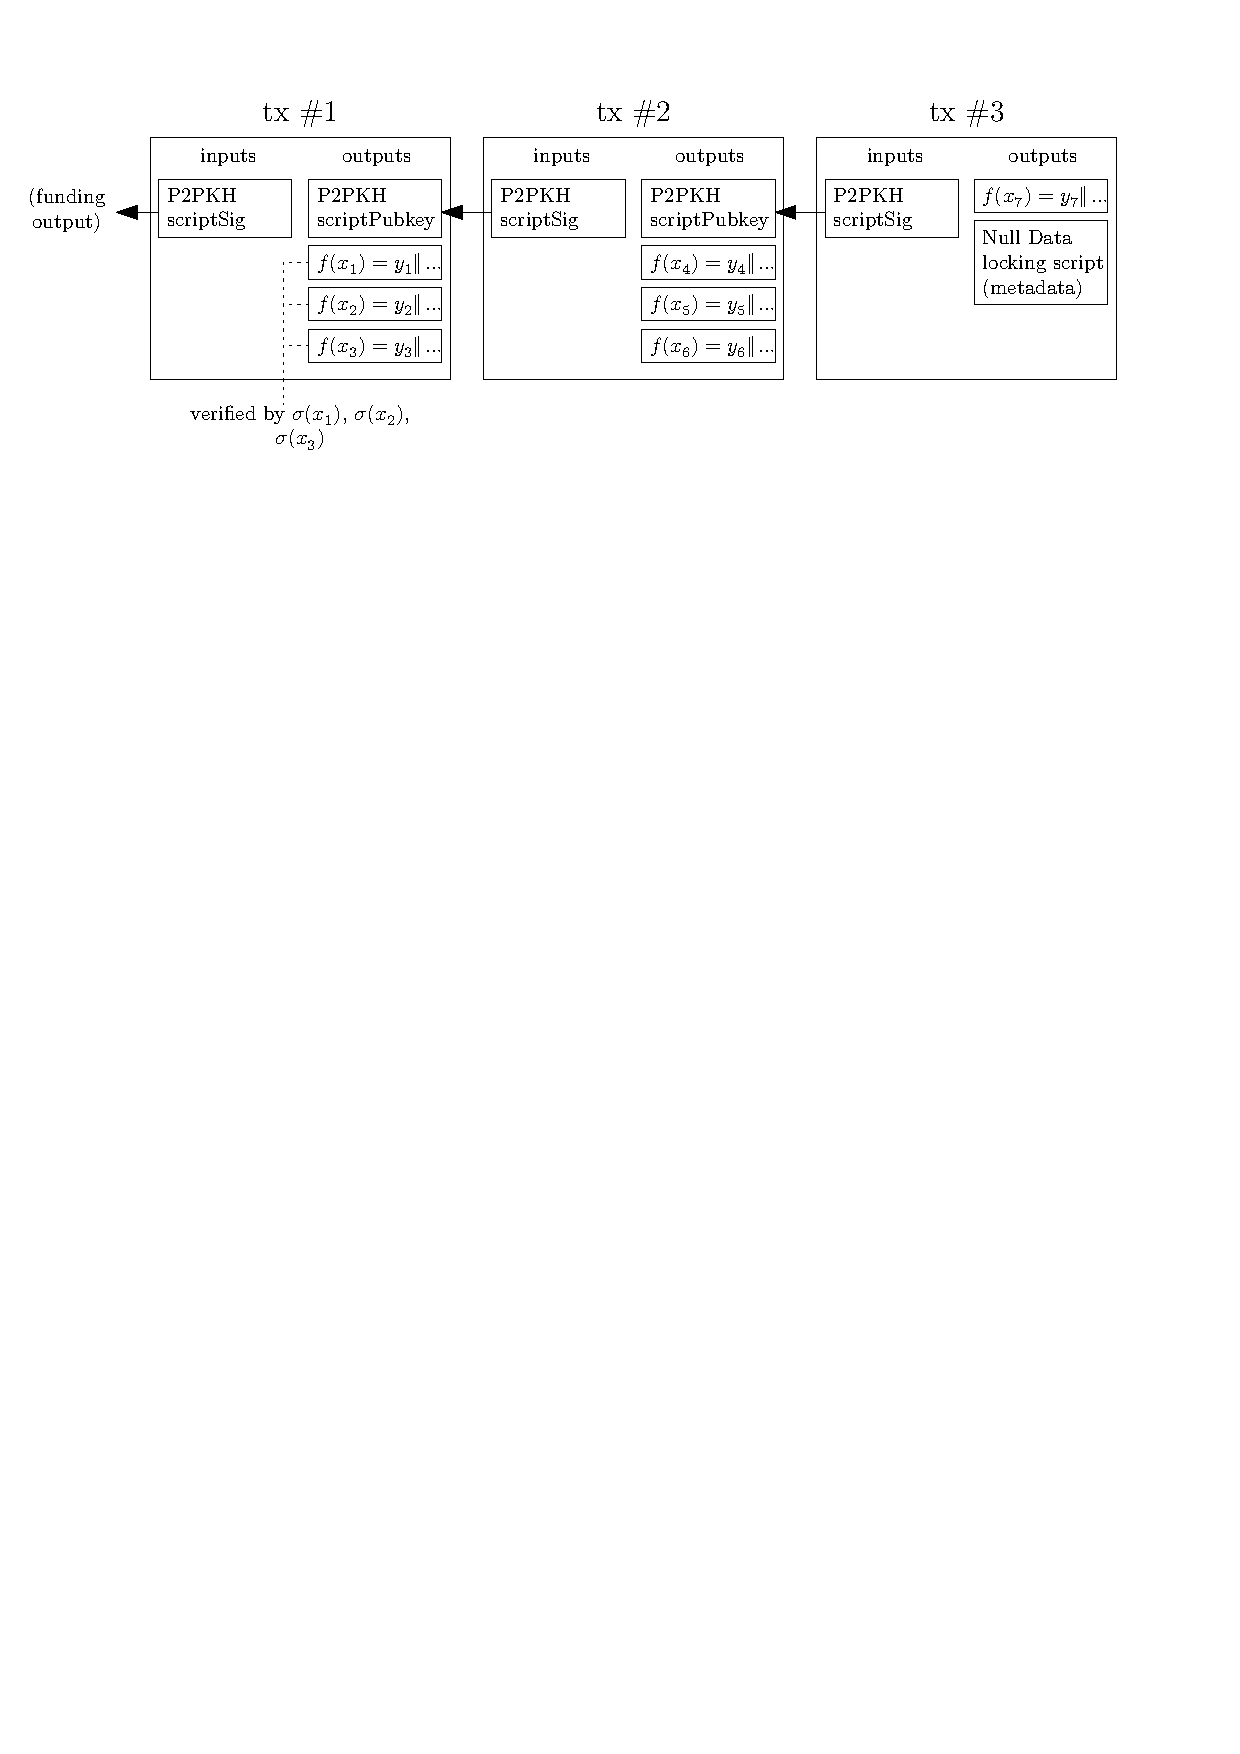
\includegraphics[width=15cm,keepaspectratio]{figure.pdf}
    \caption[Proposed scheme to construct transaction from the prepared addresses to circumvent the countermeasure]{Proposed scheme to construct transaction from the prepared addresses, which are partial preimages of the payload's fragments. Submitting tx \#1, \#2, \#3 together with the respective proofs $\sigma(x_1), \dots, \sigma(x_7)$ would then circumvent the countermeasure. Arrows from input to output signify which output the respective input is referencing; that is, the \emph{logical} direction is from right to left, the \emph{chronological} direction from left to right. Usually, more than three payload-holding outputs can be bundled into a single transaction.}
    \label{fig:tx-construction}
\end{figure}

Having provided a framework showing the theoretical possibility to circumvent such countermeasure, following section describes the necessary steps to perform such inclusion in practice.
That is, including payload data into the blockchain, where the data is embedded into ordered output addresses of transactions.
Additionally, following procedure generates private keys to each of the used output addresses, such that proofs of ownership can be deduced as required by the countermeasure, and hence the generated transactions are approved.
It is to be noted, that, in the context of Seeg's proposal, investing in a rainbow table could significantly increase performance in comparison to a full brute force approach.
Nevertheless, we omit rainbow tables, since this issue could easily be solved by refining the countermeasure, e.g.\@ including transaction hash in the proof message $m$ to be signed.
Cf.\@ the \textquote{freshness property} in the approach proposed by Matzutt et al.\@ \cite[368--369]{matzutt_thwarting_2018}.

The procedure is given with a chosen prefix length $n$. Performance and cost directly depend on this parameter, and a fit choice for $n$ is discussed in the next section.
Without loss of generality, we assume the payload length to be a multiple of $n$.

\subsubsection*{Detailed Description of the Procedure}

\emph{Preparation.} First, we split the payload into fragments $y_1, y_2, \dots, y_p$ of length $n$, and use a binary tree as efficient data structure to access the fragments, sorting them by their lexicographic order.

\emph{Partial preimage loop.}
Then, we have to find a suitable partial preimage $x_i$ for every fragment $y_i$ with $1\leq i \leq p$ in the tree.
In each iteration (of the outer loop), we generate many private key candidates $x$ by brute force (inner loop), until the prefix of $f(x)$ matches any fragment remaining in the tree.
We then can assign matching fragment $y_i$ the private key $x_i \coloneqq x$, and remove $y_i$ from the tree.
This leads to a mapping $y_i \mapsto x_i$ for all $1\leq i\leq p$.

The implementation is trivial for the P2SH method: let $s$ be an injective function transferring a nonce $m\in\mathbb{N}$ into a valid redeem script.
We start off with a random nonce $m$, and test $H(s(m))$, increment $m$, test again, and so forth.
Having found $m$ with prefix of $H(s(m))$ matching one fragment $x_i$ in the tree, we can assign that fragment the private key $s(m)\eqqcolon x_i$.
Observe that, in order to circumvent this specific countermeasure, $s(\cdot)$ must not necessarily map to a syntactically \emph{valid} redeem script, but % TODO
%Nevertheless, it is beneficial to let $s(\cdot)$ implement a redeem script testing authenticity (e.g.\@ check against a public key) to prevent the payload-holding outputs to be spent.

In the case of the P2PK/P2MS method, this translates to testing products $m\cdot G$, $(m{+}1)\cdot G$, $(m{+}2)\cdot G,\dots$ from random starting nonce $m$.
Using the axioms of the group formed by the elliptic curve, we can avoid costly elliptic curve multiplications: starting with random nonce $m$, we cache public key $P\coloneqq m\cdot G$.
When incrementing $m$, we add generator point to $P$, that is $P\coloneqq P+G$, and ensure invariant $P= m\cdot G$.
Again, having found $m$ with prefix of $P$ matching one fragment $x_i$ in the tree, we assign that fragment private key $m\eqqcolon x_i$.
The P2PKH method can be implemented similarly, by testing hashes $H(P)$.

\emph{Transaction construction.}
From assigned private keys, we can construct transactions containing the respective public keys $f(x_1), f(x_2), \dots$ in order, embedding the prefixes $y_1, y_2, \dots$.
That is, we construct a transaction with a single funding input, and add corresponding outputs containing the public keys as destination addresses, whereas every output must send a value of at least the non-dust amount with respect to the constructed output. (In the case of P2MS, up to three public keys can be merged into one output.)
This non-dust amount is required by the network rules, as otherwise the transactions will not be relayed.
The precise value is explained in Section \ref{sec:parameters}.


If the size of the transaction exceeds a defined limit, we add an output referenced by the next transaction as funding input, which contains the remaining public keys. This recursive procedure generates a chain of transactions, as depicted in Figure \ref{fig:tx-construction}.
This also ensures that the network limit of \SI{100}{\kilo\byte} per transaction is followed.
A terminal Null Data output allows embedding of metadata (such as method used, total payload length, prefix length), facilitating reconstruction of the payload.
Since we have chained the transactions using funding inputs, the transaction identifier of the last transaction can serve as locator for the data in the blockchain.
It is recommended to use P2PK(H) scripts as funding inputs, since the signatures in the respective unlocking scripts parts effectively prevent modifications to the transaction, for example an unwanted reordering of the transaction outputs.

\emph{Signature generation and submission.}
Again, having the private keys $x_1, x_2, \dots$, it is trivial to generate the proofs confirming ownership, e.g.\@ the signatures as defined by the proposed proof-of-ownership countermeasure.
Submitting both the proofs and the previously generated transaction then successfully embeds the entire payload into the blockchain.
Note that this approach allows for the payload to be split up between multiple blocks in the blockchain.

\subsubsection*{Computational Properties}

We carefully ensured that the inner iterations of the partial preimage loop, the major part constituting the computational hardness, is particularly efficient, especially by using a binary tree to quickly search for matching fragments, and caching the elliptic curve point $P$.
Hence, it seems unlikely that modifications on the iterations could increase performance (by more than a constant factor).

Likewise, it is plausible that the performance of this algorithm cannot be considerably increased.
Any other modifications would need to employ sophisticated techniques to limit the search space of potential nonces, which would directly attack the underlying cryptographic primitives (SHA256 and elliptic curve cryptography).

We further observe that the preimage loop can easily be parallelized on multiple cores and computers, especially allowing efficient implementations on GPUs.

\subsubsection*{Overview of the Implementation}

The accompanied C code implements the above mentioned procedure, split into two separate components: \emph{hidedata} performs the preparation and the partial preimage loop and outputs suitable keypairs; \emph{buildtx} then constructs the transactions from these keypairs, with assistance from the RPC interface of the Bitcoin daemon.
Furthermore, a program \emph{parsedata} allows for the reconstruction of the included data by giving as input the hash of the transaction containing the metadata (e.g.\@ the rightmost transaction in Figure \ref{fig:tx-construction})

As a proof of concept, \emph{hidedata} implements the brute-force loop without major optimizations: for both the elliptic-curve arithmetic and the hash operations the OpenSSL libraries are invoked, with a parallelization onto all CPU cores via OpenMP. Cf.\@ \texttt{src/hash\_method\allowbreak\_p2pk.c}, \dots\texttt{\_p2sh.c}, \dots\texttt{\_p2pkh.c}.
Further improvements in efficiency are considered out of scope for this implementation, since they are extremely specific to hardware and elliptic-curve theory.
Section \ref{sec:parameters} will introduce software that is optimized for these types of brute-force tasks, which compute significantly faster, parallelizing onto the GPU, and specifically in the case of elliptic-curve arithmetic, exploits the symmetry and two endomorphisms of the elliptic-curve group \cite{vanitysearch_2019}, \cite{hashcat_2020}.
Nevertheless, these software programs cannot be immediately applied to the stated problem of data inclusion, and furthermore only increase the performance by a constant factor.

The program \emph{buildtx} receives a list of keypairs and the constructs the suitable transactions as was outlined previously.
Due to the linkage between the desired transactions, the hash of the first transaction (chronologically speaking, e.g.\@ tx \#1 from Figure \ref{fig:tx-construction}) needs to be determined.
This requires the transaction to be final, hence the program communicates with the Bitcoin client via the RPC interface to let the client fund and sign the first transaction.

We omit the step of proof construction, as the generation is specific to the countermeasure implementation, yet trivial given the keypairs previously generated.
After submission into the blockchain (e.g.\@ via the Bitcoin RPC client), the included data can be reconstructed using the program \emph{parsedata}.
Taking as input the hash of the metadata-holding transaction, the program fetches all relevant transactions via the RPC interface, by following the funding references along the logical direction.
Then, using the metadata, the payload can be trivially reconstructed from the outputs of the respective transactions.


\chapter{Increased Cost of Data Inclusion}\label{chap:evaluation}

After having demonstrated the possibility to circumvent the proposed countermeasure by brute force, this section attempts to evaluate the effectiveness of that countermeasure by taking into consideration the computational cost of the circumvention.
We assume a (not necessarily adversarial) user, attempting to use the blockchain as data storage.
We will see that the user's chosen prefix length for the partial collisions directly determines the inclusion cost, hence we first model the inclusion cost mathematically. Then, by giving further estimations of essential parameters, we are able to predict by which factor the proposed countermeasure using proof-of-ownership signatures increases inclusion cost with respect to current, unprotected situation using fake addresses, as presented in Section \ref{sec:fakekeys}

\section{Modeling Inclusion Cost}

Essentially, the choice of a suitable prefix length is a trade-off:
On the one hand, the number of required keypairs, and hence needed publication cost, are inversely proportional to the chosen prefix length;
on the other hand, the probability for a partial collision decreases exponentially with respect to the prefix length, and in turn, computation cost increases exponentially.

To precisely model the cost of an inclusion of an arbitrary payload into the blockchain, restricted with the proposed countermeasure, let us denote
\begin{itemize}[noitemsep]
    \item prefix length with $n$,
    \item payload length with $N$,
    \item cost of a single hash operation with $c$,
    \item publication cost for a single address with $f$.
\end{itemize}
Moreover, we denote $m=N/n$ as the number of required addresses, (or equivalently, the number of payload fragments) and $X$ as the random variable of required hash operations.
From this, total cost $C$ of an inclusion can be given with
\[ C =  c X + fm = c X + fN/n . \]

To precisely determine random variable $X$, we remind ourselves of the general iterative procedure of the brute-force algorithm:
In each iteration, the algorithm determines a keypair such that its prefix matches one of the payload fragments not yet assigned a keypair, and then assigns that fragment the keypair.
That is, in iteration $i$, the algorithm chooses private keys randomly, until generated public key partially collides with one of the $m-i$ remaining unassigned payload fragments.
In the worst case, all fragments are pairwise different, hence one iteration can be viewed as repeated independent Bernoulli trials until success (i.e.\@ partial collision found), with success probability $(m-i)/2^n$.
Referring to required hashes in iteration $i$ with $X_i$, we thus observe that the random variable $X_i$ follows a geometric distribution with parameter $(m-i)/2^n$.
For the total number of required hash operations $X$, we reach (with $H_m$ the $m$-th harmonic number)
\[ X = \sum_{i=1}^{m} X_i, \quad E[X] = \sum_{i=1}^{m} E[X_i] = \sum_{i=1}^{m}\frac{2^n}{i} = 2^n\, H_m, \]
and conclude for the expected total cost $C$
\begin{equation}
    E[C] = 2^n\, H_m\,c + fm.\label{eq:totalcost}
\end{equation}

\section{Estimation of Parameters}\label{sec:parameters}

Before we can determine the cost increase caused by the proposed countermeasure, we need to give sensible estimations for the cost parameters $c$ and $f$ involved in the previously stated cost model (Eq.~\ref{eq:totalcost}).
While publication cost $f$ of an address are directly determined by the miners' transaction fee rate and bitcoin price, hashing cost depends on the efficiency of the hardware used for the brute-force process.
For this, we estimate the parameter indirectly using hashrates reported by users of the tools \emph{VanitySearch} by Pons \cite{vanitysearch_2019} and \emph{Hashcat} by Steube et al.\@ \cite{hashcat_2020}.

\subsubsection*{Transaction Fees and Burnt Coins}


\begin{table}[t]
    \centering
    \begin{tabular}{lrrrS[table-format=0.8,table-alignment=right]rS[table-format=2.1e-1,table-alignment=right]}
        \toprule
        & \llap{\textbf{script}} & \textbf{payload} & \textbf{addresses} & {\textbf{total cost}} & {} & {}\cr
        \textbf{Type} & \textbf{size} & \textbf{length} & {\textbf{per tx}} &  {\textbf{in BTC}} & {\textbf{$f$ in sat}} & {\textbf{$f$ in USD}}\cr
        \midrule
        P2PK         & 35 B & 32 B& 2267 &    0.03305332 &1458.02 & 14.6e-2\cr
        1-of-3 P2MS  & 105 B & 32 B& 2625 &   0.02687330 &1023.74 & 10.2e-2\cr
        P2PKH        & 25 B& 20 B & 2934 &    0.03601664 &1227.56 & 12.3e-2\cr
        P2SH         & 23 B& 20 B & 3117 &    0.03682640 &1181.47 & 11.8e-2\cr
        1-of-3 P2FMS & 201 B & 65 B& 1425 &   0.02509730 &1761.21 & 17.6e-2\cr
        \bottomrule
    \end{tabular}
    \caption[Overview of the different transaction types]{Overview of the different transaction types.
        Second column denotes the scripts size for a transaction output, holding an address (resp.\@ three addresses in the case of multisig), third column the maximum payload length per address.
        Fourth column gives how many addresses can be gathered in a single transaction (not exceeding the size limit of \protect\SI{100}{\kilo\byte}), fifth column the total cost for submitting this transaction, that is with smallest non-dust amount (depending on transaction type) per output plus transaction fees of 20 sat per byte.
        Value $f$ is obtained by dividing total cost by number of addresses, further assuming current exchange rate of \num{10000} USD per BTC.}
    \label{table:txtypes-parameters}
\end{table}

The cost required for publishing the address into the blockchain, i.e.\@ parameter $f$, can be estimated using average bytes required for a transaction output.
First observe, that besides transaction fees (proportional to transaction size), each output must hold a minimum \emph{non-dust} value such that the transaction is relayed by the network.
Approximately, a non-dust value is larger than the transaction fees required for spending the output.
Specifically, the value depends on the output's script size $l$ and is defined as $(\SI{157}{\byte} + l)\cdot 3\,\text{sat}\,\si{\per\byte}$.

While under the conditions of the intended inclusion attack, the attacker has control of the private keys corresponding to the spent non-dust amounts, nevertheless, these coins are effectively non-recoverable and hence burnt: in order for the recovery to be economically beneficial, transaction fees required for the recovery need to be lower than the non-dust amount recovered.
We tacitly assume that at least one signature is present in each unlocking script (as otherwise the locking scripts were not secured), hence the unlocking scripts have each length at least $\SI{71}{\byte}$. Combined with the fact that the smallest output script has length $\SI{23}{\byte}$ (P2SH type), we obtain that transaction fee for the recovery transaction needs to be $\num{<5.2}$ sat per byte, as otherwise fees exceed the funds recovered.

Under these constraints, the recovery transaction competes with many transactions having larger transaction fee, and conclusively, inclusion into a mined block is extremely unlikely.
(Observe that for P2MS-spending transactions, fee per sigop cost – instead of size – determines position in the mempool. Under these conditions, an economic recovery transaction competes with even more transactions, having fee $\num{>2}$ sat per byte.)


Now, in order to obtain parameter $f$, we construct the largest possible transaction  using a single P2PK coinbase input to fund the outputs with non-dust burns, and adding outputs until reaching network's size limit of $\SI{100}{\kilo\byte}$.
Multiplying with miner's transaction fees, and adding the smallest respective non-dust burn amount to each output yields the value for parameter $f$.
Table \ref{table:txtypes-parameters} gives this parameter in absolute values for all three methods, using transaction fees of 20 sat per byte (identical to \cite{sward_data_2018}), and Bitcoin exchange rate at point of writing (\num{10000} USD per bitcoin).
Note that the P2MS strategy, arranging pubkeys in 1-of-3 multisig outputs, is currently the least expensive one with respect to $f$.
Even though multisig outputs cause more overhead in the constructed transaction, required non-dust amount is lower per output, hence, grouping three pubkeys into one transaction output saves on burnt bitcoins.


\subsubsection*{Hash Cost Estimation}
\begin{table}[t]
    \centering
    \begin{tabular}{lr<{\,\si{\watt}}S[table-format=4.0,table-number-alignment=right]@{\,}rS[table-format=1.2e-2,table-number-alignment=right]l}
        \toprule
        \textbf{Hardware} & \multicolumn{1}{r}{\textbf{wattage}} &\multicolumn{2}{r}{\textbf{est.\@ freq.}} & \multicolumn{1}{r}{\textbf{$c$ in USD}} & \textbf{ref.}\cr
        \midrule
        \emph{P2PKH} \cr
              GTX 1660 TI  & 120 & 960 & \si{\mega\hertz} & 4.51e-15 &  \cite[][\#396]{forums_vanitysearch}\cr
              GTX 1650  & 75 & 510 & \si{\mega\hertz} & 5.31e-15 &  \cite[][\#374]{forums_vanitysearch}\cr
              RTX 2080 Super  & 250 & 2000 & \si{\mega\hertz} & 4.51e-15 &  \cite[][\#396]{forums_vanitysearch}\cr
              RTX 2080 TI (MSI) & 300 & 2500 & \si{\mega\hertz} & 4.33e-15 &  \cite[][\#343]{forums_vanitysearch}\cr
              Tesla V100-SXM3-32GB  & 300 & 2500 & \si{\mega\hertz} & 4.33e-15 &  \cite[][\#619]{forums_vanitysearch}\cr
        \midrule
        \emph{P2SH} \cr
        GTX 1080 TI & 250 & 2400 & \si{\mega\hertz} & 3.76e-15 & \cite{gosney_1080ti} \cr
        RTX 2080 TI & 300 & 3700 & \si{\mega\hertz} & 2.93e-15 &\cite{celik_2080ti} \cr
        \bottomrule
    \end{tabular}
    \caption[Selected user's reports of their brute-force frequencies on specific hardware]{Selected user's reports of their brute-force frequencies on specific hardware. For the P2PKH method, frequency was directly taken from reported \emph{VanitySearch} speeds. For the P2SH method, SHA256 hash frequency reported from \emph{Hashcat} was divided by factor 2, as explained in the respective section.
    We estimate cost parameter $c$ for the {P2PKH} by first researching estimated power consumption of the GPU under full load, and assuming energy cost of \num{.13} USD per \si{\kilo\watt\hour}.}
    \label{table:cost}
\end{table}

For the {P2PKH} method, we can rely on user reports on their performance using the tool \emph{VanitySearch}, which allows users to create \emph{vanity addresses}.
These Bitcoin addresses contain a human-readable message as prefix in their Base-58 representation; cf.\@ \cite[82--83]{antonopoulos_mastering_2017}.
Similarly to the presented tool in previous section, \emph{VanitySearch} brute-forces private keys, until the hashed public key has the desired prefix;
this public key hash is precisely the one used to create {P2PKH} hashes.

Hence, due to the computational similarity, it seems reasonable to estimate possible computational cost for the {P2PKH} method from reported frequencies of \emph{VanitySearch} on selected hardware.
We assume that the computational effort of testing if a public key hash partially collides with one of the remaining unassigned payloads is negligible.
Table \ref{table:cost} gives estimations for cost $c$ bases on selected user reports form the \emph{Bitcointalk} forums.
We assume an energy cost of \num{.13} USD per \si{\kilo\watt\hour}.

In a similar matter, one can use the performances in computing {SHA256} digests as estimation for the cost of the {P2SH} method.
As was outlined in previous section, the brute-force procedure for the {P2SH} method constructs from nonce candidate $x$ a 57-byte long redeem script $s(x)$, and computes the {P2SH} address as the hash digest $H(x)$, that is by definition
\begin{equation}
    x \mapsto \text{{RIPEMD160}}(\text{{SHA256}}(s(x))).\label{eq:p2sh-hash}
\end{equation}
The primitive hash functions {RIPEMD160} and {SHA256} are highly similar in architecture and performance; their respective Merkle–Damgård transforms also operate on the same block size of 512 bits.
Cf.\@ for example the \emph{ECRYPT Benchmarking of Cryptographic Systems} \cite{bernstein_benchmark}.
Therefore, the effort required in above procedure (Eq.~\ref{eq:p2sh-hash}) can be considered twice as large as one {SHA256} digest computation (in the sense of input length $\leq\!\SI{512}{\bit}$).

Likewise to previous estimation using \emph{VanitySearch}, we can use hash frequencies published by users of the password cracking tool \emph{Hashcat}.
Dividing the reported SHA256 hash frequency by factor 2 thus yields an approximate frequency accomplishable for the P2SH brute-force procedure.
(We can assume that the GPU can be programmed to perform RIPEMD160 calculations in similar speed.)
Again, refer to Table \ref{table:cost} for estimations on cost $c$ bases on selected user reports.
These numbers should explicitly not be understood to represent the current state of hardware efficiency, but rather as figures attainable with available off-the-shelf hardware.
While non-GPU hardware has the potential to be more energy-efficient, either the hardware cannot be easily adapted (e.g.\@ in the case of ASIC hardware), or the frequencies are too low to perform the brute-force algorithm in sensible time.

Both the P2PKH and the P2SH method perform the same hash operations, only the former has to additionally perform an elliptic-curve addition.
Comparing the two methods, we can already observe that the digest calculation in the P2PKH method significantly contributes to total computation time, next to the elliptic-curve arithmetic.

Nevertheless, specialized software for cracking ECDSA keypairs does not appear to exist, hence we cannot estimate parameter $c$ in the same manner.
We therefore omit a precise cost estimation of the P2PK/P2MS method, and use the cost parameter $c$ of the P2PKH method as upper bound.

\section{Comparison with State-of-the-Art Methods}\label{sec:comparison}

\begin{figure}[tb]
    \centering
    \pgfplotstableread[col sep=comma, ignore chars={"}]{plot1.csv}{\totalcostplot}
    \begin{tikzpicture}[
            mark size=1.5pt
        ]
        \begin{semilogyaxis}[
                height=8cm,
                width=13cm,
                grid=both,
                xmin=5,
                xmax=60,
                ymax=400,
                log ticks with fixed point,
                ymin=1,
                cycle list name=mylist,
                legend style={at={(0.5,0.95)},
		anchor=north,legend columns=2},
                xlabel={Prefix length $n$ in bits},
                ylabel={Expected cost in USD per kilobyte}
            ]

            \addplot+[mark=x] table [x={n}, y={p2pk}] {\totalcostplot};
            \addlegendentry{P2PK}
            \addplot+[mark=o] table [x={n}, y={p2ms}] {\totalcostplot};
            \addlegendentry{P2MS}
            \addplot+[mark=triangle] table [x={n}, y={p2pkh}] {\totalcostplot};
            \addlegendentry{P2PKH}
            \addplot+[mark=square] table [x={n}, y={p2sh}] {\totalcostplot};
            \addlegendentry{P2SH}
            \addplot+[dashed,mark=none] table [x={n}, y={p2fms}] {\totalcostplot};
            \addlegendentry{fake multisig}
        \end{semilogyaxis}
    \end{tikzpicture}
    \caption[Log-linear plot of expected total cost]{Log-linear plot of expected total cost $\mathrm{E}[C]$ (see Equation \ref{eq:totalcost}) with $N=\protect\SI{10}{\kilo\byte}$ for inclusion methods P2PKH ($c=\num{4.50e-15}$ USD, $f=\num{12.3e-2}$ USD), P2MS ($c=\num{4.50e-15}$ USD, $f=\num{10.2e-2}$ USD), P2SH ($c=\num{3.0e-15}$ USD, $f=\num{11.8e-2}$ USD). For comparison, dotted line indicates constant efficiency achievable using fake addresses in multisig outputs (P2FMS).}
    \label{fig:plot}
\end{figure}

This section compares the impact of the proposed inclusion method with the current situation, having no countermeasures.
To begin with, we choose the following rough but sensible estimates for computation cost parameter $c$ for methods P2MS, P2PKH, P2SH, based on our observations from previous section.
We estimate $c_\text{ms}=c_\text{pkh}=c_\text{p2pkh}=\num{4.50e-13}$ USD, $c_\text{sh} = \num{3.00e-15}$ USD.
Also stated in previous section, publication cost parameter $f$ directly follows from Bitcoin exchange rate and mining fees, and is displayed in Table \ref{table:txtypes-parameters}.

From the results of Sward et al.~\cite[cf.~Table 3]{sward_data_2018}, we can infer that the best present method of including arbitrary data using fake addresses exploits fake public keys (in their extended 65 byte representation) arranged in 1-of-3 multisig outputs, not being inhibited by any countermeasure requiring proof signatures (P2FMS).
Relative cost of inclusion using this state-of-the-art method can easily be estimated using same formula (Eq.~\ref{eq:totalcost}), assigning $c=0$, maximum prefix size $n=\SI{65}{\byte}$, and computing $f$ identically to previous procedure (see also Table \ref{table:txtypes-parameters}).
This gives us a constant cost efficiency of \num{2.71} USD$\,\si{\per\kilo\byte}$ as benchmark.

Figure \ref{fig:plot} plots the expected cost per byte payload, with respect to prefix length $n$, using $N=\SI{10}{\kilo\byte}$ and previously stated parameters, for each method.
As comparison, the constant relative cost of the state-of-the-art method is highlighted by the dashed horizontal line.

Observe that, for each method, the local minimum of the respective cost function corresponds to optimal (i.e.\@ cheapest) prefix length for that method.
Furthermore, the plot confirms the trade-off nature of the problem: left of the minimum point, cost increases proportional due to more addresses required; cost right of the minimum point is dominated by the exponentially increasing brute force computation cost.

We give minimum cost per kilobyte payload in Table \ref{table:optimalcost}, and obtain following result:
defending the Bitcoin network against unwanted data inclusion using proof-of-ownership signatures could allow for an 6-fold increase of inclusion cost, at current situation.

It needs to be highlighted that optimal cost efficiency can only be obtained using significant computation time.
For example, using the fastest GPU for the P2SH inclusion method from Table \ref{table:cost}, performing the brute-force algorithm with \SI{10}{\kilo\byte} payload already requires more than 169 hours of computation.
In order to reduce the computation time while maintaining optimal cost, one would need to parallelize multiple processing units of same cost efficiency.

Nevertheless, real-time inclusion using non-specialized hardware seems out of reach for prefix lengths as low as 28 bits, requiring more than a minute of computation time on a typical personal computer for payload length of $N=\SI{100}{\byte}$ (assuming hash frequency of \SI{10}{\mega\hertz}).

\begin{table}
    \centering
    \begin{tabular}{lrS[table-format=2.1,table-alignment=right]S[table-format=1.2,table-alignment=right]}
        \toprule
        & {\textbf{\llap{opt.\@ prefix}}} & {\textbf{exp.\@ cost in}} & \textbf{{rel.\@ increase}}\cr
        & {\textbf{length}} & {\textbf{USD per kB}} & {\textbf{w.r.t.\@ P2FMS}}\cr
        \midrule
        P2PK  & 48 & 35.3 & 9.34\cr
        P2MS  & 47 & 17.9 & 6.61\cr
        P2PKH & 47 & 21.4 & 7.90\cr
        P2SH  & 48 & 20.4 & 7.52\cr
        \bottomrule
    \end{tabular}
    \caption[Minimum expected cost]{Minimum point $n$ and minimum value $\mathrm{E[C]}$ from plot in Figure \ref{fig:plot}. Rightmost column gives the relative increase with respect to the constant efficiency achievable using fake addresses in multisig outputs.}
    \label{table:optimalcost}
\end{table}



\section{Variations in Parameters}

\begin{figure}[p]
    \centering
    \pgfplotstableread[col sep=comma, ignore chars={"}]{plot2-fit.csv}{\costfit}
    \pgfplotstableread[col sep=comma, ignore chars={"}]{plot2-points.csv}{\costpoints}
    \pgfplotstableread[col sep=comma, ignore chars={"}]{plot3-fit.csv}{\relfit}
    \pgfplotstableread[col sep=comma, ignore chars={"}]{plot3-points.csv}{\relpoints}
    \begin{tikzpicture}[
            mark size=1.5pt
        ]
        \begin{loglogaxis}[
                height=8cm,
                width=13cm,
                grid=both,
                cycle list name=mylist,
                legend style={at={(0.99,0.01)},
                anchor=south east,legend columns=1},
                xlabel={Bitcoin price $p$ in USD},
                ylabel={$C_\mathrm{p2ms}(c,f)$ in USD per kilobyte}
            ]

            \addplot+[] table [x index={0}, y index={1}] {\costfit};
            \addlegendentry{$c=\SI{10e-14}\,\text{USD}$}
            \addplot+[] table [x index={0}, y index={2}] {\costfit};
            \addlegendentry{$c=\SI{10e-16}\,\text{USD}$}
            \addplot+[] table [x index={0}, y index={3}] {\costfit};
            \addlegendentry{$c=\SI{10e-18}\,\text{USD}$}
            \addplot+[] table [x index={0}, y index={4}] {\costfit};
            \addlegendentry{$c=\SI{10e-20}\,\text{USD}$}
            \addplot+[] table [x index={0}, y index={5}] {\costfit};
            \addlegendentry{$C_\mathrm{fake}(p)$}
            \pgfplotsset{cycle list shift=-5}
            \addplot+[mark=+,only marks] table [x index={0}, y index={1}] {\costpoints};
            \addplot+[mark=+,only marks] table [x index={0}, y index={2}] {\costpoints};
            \addplot+[mark=+,only marks] table [x index={0}, y index={3}] {\costpoints};
            \addplot+[mark=+,only marks] table [x index={0}, y index={4}] {\costpoints};
        \end{loglogaxis}
    \end{tikzpicture}\\[3em]
    \begin{tikzpicture}[
            mark size=1.5pt
        ]
        \begin{loglogaxis}[
                height=8cm,
                width=13cm,
                grid=both,
                ytick={4,5,6,7,8,9,10},
                yticklabels={4,5,6,7,8,9,10},
                cycle list name=mylist,
                legend style={at={(0.05,0.95)},
                anchor=north west,legend columns=1},
                xlabel={Bitcoin price $p$ in USD},
                ylabel={$C_\mathrm{p2ms}(p,c)/C_\mathrm{fake}(p)$},
            ]

            \addplot+[mark=+] table [x index={0}, y index={1}] {\relfit};
            \addplot+[mark=+] table [x index={0}, y index={2}] {\relfit};
            \addplot+[mark=+] table [x index={0}, y index={3}] {\relfit};
            \addplot+[mark=+] table [x index={0}, y index={4}] {\relfit};
            \pgfplotsset{cycle list shift=-4}
            \addplot+[mark=+,only marks] table [x index={0}, y index={1}] {\relpoints};
            \addplot+[mark=+,only marks] table [x index={0}, y index={2}] {\relpoints};
            \addplot+[mark=+,only marks] table [x index={0}, y index={3}] {\relpoints};
            \addplot+[mark=+,only marks] table [x index={0}, y index={4}] {\relpoints};
        \end{loglogaxis}
    \end{tikzpicture}
    \caption[Optimal relative inclusion cost with respect to arbitrary parameters $c$ and bitcoin price $p$]{Top figure plots the optimal relative inclusion cost for the P2MS method with respect to fixed parameter $c$ and variable bitcoin price $p$ in a log-log scale. For comparison, red line shows the linear relative inclusion cost using fake keys.
    Marked points denote numerically determined values, while the respective lines show the fit specified by the established regression model. Bottom figure is set up identically, but plots the respective effect factor of the countermeasure, i.e.\@ the relative increase of inclusion cost with respect to P2FMS.}
    \label{figure:fit}
\end{figure}

We established a model estimating cost of inclusion from parameters $N$, $f$ and $c$, corresponding to payload size resp.\@ the economic situation of the Bitcoin network (transaction fees, bitcoin exchange rate) resp.\@ computational cost of the hashing procedure.
It is therefore logical to investigate the impact on changes on this parameter, especially since a continuation of the exponentially growing trend of computation efficiency is expected.
To keep the analysis reasonable, we restrict the parameter space to $10^{-20} \leq c \leq 10^{-14}$ for computation cost, and for the bitcoin price $p$ to range $10^3\,\text{USD}/\text{BTC} \leq p \leq 10^6\,\text{USD}/\text{BTC}$.
Due to the transcendental nature of the cost function $\mathrm{E}[C]$ with respect to prefix length $n$, it seems out of reach to formulate a closed-form solution to finding optimal prefix length and respective total cost, given parameters $N$, $f$, $c$.
Hence, numerical methods are applied to determine minimal cost, given numerical values of the parameters.

Before discussing the impact of $p$ and $c$, we can observe that relative savings from larger payload size $N$ are effectively negligible, that is, total cost is near-linear with respect to payload size;
this trend is independent of all other parameters.
Therefore, we continue our analysis by looking at the cost of an inclusion \emph{relative} to payload size, while additionally fixing $N=\SI{10}{\kilo\byte}$.

In order to derive parameter $f$ from bitcoin exchange rate $p$, we fix the P2MS method and network transaction fees of 20 sat per byte.
This is motivated by the fact that 20 sat per byte can be considered a lower bound on the network's transaction fee, and assuming this value, P2MS method is the cheapest one.
Accordingly, the final results of the following calculation can be interpreted as a reasonable lower bound.

As was already performed in Section \ref{sec:parameters}, we can define parameter $f$ in units of sat, and multiply with $p$ to obtain parameter $f$ in terms of USD.
Combining with given parameter $c$, let $C_\text{p2ms}(p,c)$ be the optimal relative inclusion cost in USD per byte, determined by numerically finding optimal prefix length $n$.
By same methods, we can generalize the inclusion cost using fake keys, as
\[ C_\text{fake}(p) = \frac{N}{\SI{65}{\byte}} \cdot f_\text{p2fms} \cdot p. \]
Cf.\@ Equation \ref{eq:totalcost} and Table \ref{table:txtypes-parameters}.

In order to state the effect of bitcoin price and computation cost quantitatively, we proceed with numerically computing $C_\text{p2ms}(p,c)$ for $c$ and $p$ in the previously fixed respective ranges; both price $p$ and $c$ in $10^{0.2}$-fold increments, yielding 416 data points.

We continue by presenting a bivariate log-log regression model to explaining the dependent data points from the independent variables, that is,
\begin{equation} \log_{10} \frac{C_\text{p2ms}(p, c)}{\text{USD}\,\si{\per\byte}} = \alpha + \beta \log_{10} \frac{p}{\text{USD}} + \gamma \log_{10} \frac{c}{\text{USD}} + \epsilon_i, \label{eq:regressionmodel}\end{equation}
with unknown parameters $\alpha$, $\beta$, $\gamma$, and error terms $\epsilon_i$.
Usual least-squares-error method provides $\alpha \approx \num{-65.292}$, $\beta \approx\num{0.97498}$, $\gamma \approx\num{.002495}$.


It is explicitly to be remarked that this model does not precisely explain the data; this becomes clear when considering the visible patterns in the residual graph of this regression.
Nevertheless, the model appears to be sufficiently precise to estimate the effect of the variables $p$, $c$ on relative inclusion cost: in fact, mean square error $< \num{e-5}$, and maximum residual is $\max |\epsilon_i| < 0.0125$. Consequently, the model predicts inclusion cost with a relative error of at most \SI{2.92}{\percent}.
See also Figure \ref{figure:fit}, which plots observed data points against the fit in a log-log plot.

Having established that model, we can derive from parameters $\beta$ and $\gamma$ following observations:
First, as we expected, relative inclusion cost $C_\mathrm{p2ms}(p,c)$ is almost linear with respect to bitcoin price $c$.
Since sub-linear, we expect that $C_\mathrm{p2ms}(p,c)$ continues to converge towards $C_\mathrm{fake}(p)$, which grows linear with respect to $p$.
Nevertheless, this trend appears to be minor; a 100-fold bitcoin price increase lowers relative inclusion cost by no more than \SI{11}{\percent}.

Second, computation cost $c$ has – independent of bitcoin price $p$ – only slim effects on inclusion cost: lowering computation cost by factor $10$, for example, would reduce relative inclusion cost by \SI{5.59}{\percent}. (Moore's law would estimate such cost decrease of factor $10$ in a time span of 7 years.)

We conclude: even though effectiveness of the proposed countermeasure decreases both with increasing bitcoin price and decreasing computational cost, effectiveness remains stable even for extreme values.
For our established bounds of parameters, this means $\num{4.3} \leq C_\mathrm{p2ms}(p,c) / C_\mathrm{fake}(p) \leq \num{7.3}$.


\chapter{Conclusion}\label{chap:conclusion}

\subsubsection*{Summary}

Section \ref{chap:problem} gave an overview of the current method to include off-topic data using fake addresses, exploiting the presence of data fields in the transaction that are essential for payment processing in honest transactions.
This exploit depends on the difficulty to verify the authenticity of (generalized) destination addresses, i.e.\@ the network cannot distinguish between honest addresses and payload data masquerading as an address.

In consideration with the (community-defined) principles of the Bitcoin network, we generalize a countermeasure proposed by Seeg.
In principle, this proof-of-ownership countermeasure considers a transaction clean if and only if the sender of that transaction has control of the private components of the destination addresses.
That is, if and only if the sender can provide signatures proving his control.
We argued in Section \ref{chap:countermeasure} that such countermeasure can be considered maximally strong with respect to the principles of the network, motivating the analysis of the effectiveness of that countermeasure.

From the considered countermeasure immediately follows a parallelizable brute-force approach to circumvent that countermeasure, outlined in Section \ref{sec:circumvention}. Section \ref{sec:design} gives an abstract overview of the implementation design.
Specifically, the implementation allows a trade-off between computation time required for generation, and cost required for publication into the network.
Furthermore, the construction generates addresses in such a way that the straightforward reconstruction of the payload data is possible.

Section \ref{chap:evaluation} gives a stochastic model that estimates the cost required by the brute-force circumvention, using the outlined implementation, assuming the presence of the considered countermeasure.
Then, required parameters (cost associated with transaction publication resp.\@ computation cost) are determined, whereas computation cost is estimated using publicly available data on hardware performance.
At the current date, the proposed countermeasure would increase the cost of arbitrary data inclusion by factor \num{6.6}.
Variations in these parameters show that this factor is in the range $[\num{4.3}, \num{7.3}]$ for realistic values, considering the best-performing P2MS method.
Furthermore, our regression model implies that inclusion cost circumventing the countermeasure is dominated by Bitcoin price in a near-linear relationship.
Impact on computing cost $c$ however is heavily sublinear, with a growth behavior proportional to $c^\gamma$, $\gamma \ll 1$ (cf.\@ Eq.\@ \ref{eq:regressionmodel}), implying that improvements in hardware lead to minor effects on the effectiveness of the countermeasure.

Besides the increase in inclusion cost, the required computation time (even if cheap, relatively speaking) might already discourage actors wishing to include arbitrary data into the blockchain.
In other words, the countermeasure ensures that a large data inclusion within a reasonable time is only possible if a lot of parallel computing power is available.

\subsubsection*{Outlook}

If inclusion of data into the blockchain were to become a major and existing problem, adoption of Seeg's countermeasure could contribute to protecting against this attack.
While the additional checks imposed by the countermeasure appear to be in accordance with the general principles of the network, it comes with drawbacks concerning general usability and increased verification work for miners.
Furthermore, a parallelization of the brute-force process might make data inclusion a feasible option for some actors.

Following our assessment that the proposed countermeasure is maximally strong with respect to the principles, we observe that the effectiveness of the countermeasure directly depends on the computational hardness of the outline brute-force algorithm.
While replacements in the underlying cryptographic primitives of Bitcoin are expected to be controversial, these could have a significant impact on the circumvention's hardness, and hence can be employed to further improve the effectiveness of the countermeasure.

For example, a sensible strengthening could be achieved by replacing the implementation of Bitcoin's script hash function $H$ to a memory-hard hash function (e.g.\@ \emph{scrypt} \cite{percival_scrypt}).
With applicable parameters, this adoption would make the parallelization of the brute-force process (memory-)costly, but without strongly impeding miners computing the hash digests during transaction verification.
Thus, combined with a ban of P2PK/P2MS transactions (i.e.\@ restricting outputs to $H$-digests), the time required to compute the respective keypairs for a data inclusion could be moved out of reasonable bounds.


Nevertheless, with the presence of the discussed countermeasure, it is unreasonable to expect an adversary attempting to deliberately insert large problematic data.
For one, even without the discussed replacement of the hash function $H$, such large-scale inclusion attack would require significant hashing power, which would be rather invested in gaining a relevant portion of the network's hashrate.

For another, the inclusion of large data would cause a significant increase in transaction fees:
as a large-scale inclusion occupies significant portions of the mined blocks, honest transactions compete for narrowed space in the blocks, causing miners to prioritize high-fee transactions.
Hence, this attack is effectively translated into a denial-of-service attack, whereas the latter can be performed by easier means.


\backmatter

\phantomsection \label{listoffig}
\addcontentsline{toc}{chapter}{\listfigurename}
\listoffigures
\cleardoublepage
\phantomsection \label{listoftab}
\addcontentsline{toc}{chapter}{\listtablename}
\listoftables

\cleardoublepage
\phantomsection \label{biblio}
\addcontentsline{toc}{chapter}{References}
\printbibliography[title=References]

\end{document}
